\documentclass[tikz,border=2pt]{standalone}
\usepackage{amsmath,amssymb}
\usepackage{tikz}

\begin{document}
% A Euclidean network: cities with plane coordinates, every pair joined by an edge whose
% length is the straight-line distance sqrt((x_i - x_j)^2 + (y_i - y_j)^2).
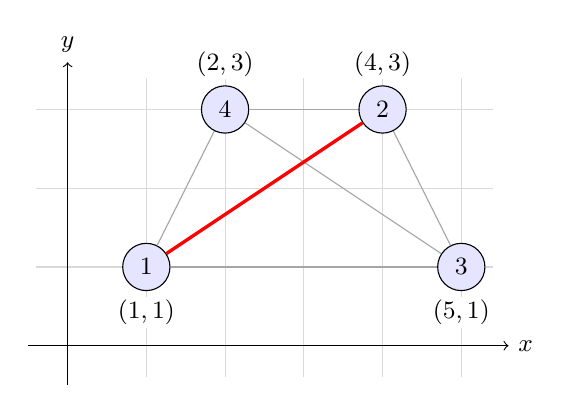
\begin{tikzpicture}[every node/.style={font=\small}, v/.style={draw, circle, fill=blue!10, minimum size=6mm, inner sep=0pt}]
	\draw[gray!30, step=1] (-0.4,-0.4) grid (5.4,3.4);
	\draw[->] (-0.5,0) -- (5.6,0) node[right, font=\small] {$x$};
	\draw[->] (0,-0.5) -- (0,3.6) node[above, font=\small] {$y$};
	\node[v] (P) at (1,1) {$1$};
	\node[v] (Q) at (4,3) {$2$};
	\node[v] (R) at (5,1) {$3$};
	\node[v] (S) at (2,3) {$4$};
	\foreach \a/\b in {P/Q, P/R, P/S, Q/R, Q/S, R/S} {\draw[gray!70] (\a) -- (\b);}
	\draw[red, very thick] (P) -- (Q);
	\node[font=\small, anchor=north, fill=white, inner sep=1pt] at (1,0.62) {$(1,1)$};
	\node[font=\small, anchor=south, fill=white, inner sep=1pt] at (4,3.38) {$(4,3)$};
	\node[font=\small, anchor=north, fill=white, inner sep=1pt] at (5,0.62) {$(5,1)$};
	\node[font=\small, anchor=south, fill=white, inner sep=1pt] at (2,3.38) {$(2,3)$};
	\end{tikzpicture}
\end{document}
